\section{Copper --- Fermi surface, orbital character of energy bands}
\label{sec4:copper}
\begin{itemize}
\item Outline: {\it Obtain MLWFs to describe the states around the Fermi-level in copper}
\end{itemize}


\begin{figure}[h!]
\centering
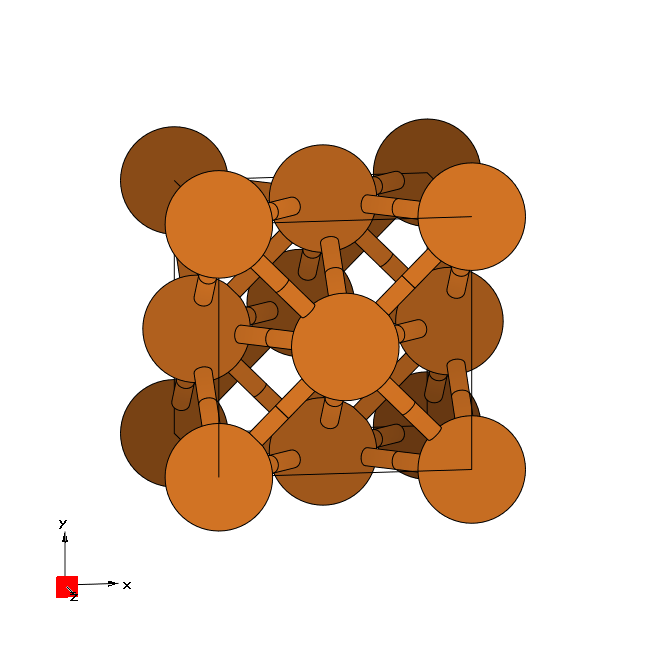
\includegraphics[width=0.25\columnwidth,trim={45pt 45pt 55pt 55pt},clip]{figure/example04/copper_crystal.png}
\caption{Unit cell of Copper crystal plotted with the \xcrysden{} program.}
\label{fig4.0}
\end{figure}

\begin{enumerate}
	\item {\it Run \Wannier{} to minimise the MLWFs spread. Inspect the output file {\tt copper.wout.}}

	Starting from 5 $d$ orbitals centred on the Copper atom and 2 $s$ orbitals in the interstitial regions of the FCC, we obtain the following spreads and centres after 200 iterations (extract from the {\tt copper.wout}, a summary of the wannierisation is given in tab.\ref{tab4.1}.):
	\begin{tcolorbox}[sharp corners,boxrule=0.5pt]
	{\small
	\begin{verbatim}
 Final State
  WF centre and spread    1  ( -0.000000,  0.000000, -0.000000 )     0.40838932
  WF centre and spread    2  ( -0.000000, -0.000000, -0.000000 )     0.30784969
  WF centre and spread    3  ( -0.000000, -0.000000,  0.000000 )     0.30784979
  WF centre and spread    4  ( -0.000000, -0.000000,  0.000000 )     0.40838973
  WF centre and spread    5  (  0.000000, -0.000000, -0.000000 )     0.30784886
  WF centre and spread    6  ( -0.902512,  0.902512,  0.902512 )     1.14385632
  WF centre and spread    7  (  0.902512, -0.902512, -0.902512 )     1.14385635
  Sum of centres and spreads (  0.000000, -0.000000, -0.000000 )     4.02804006

         Spreads (Ang^2)       Omega I      =     3.662691490
        ================       Omega D      =     0.001894482
                               Omega OD     =     0.363454087
    Final Spread (Ang^2)       Omega Total  =     4.028040058
 ------------------------------------------------------------------------------
	\end{verbatim}
	}
	\end{tcolorbox}
	We can readily see that looking at the individual spreads we find two groups of \MLWFs, a group of 5 $d$-like \MLWFs{} centred on the Copper atom, whose spreads are $0.4084$\angsqd and $0.3078$\angsqd respectively, and a group of 2 $s$-like \MLWFs{} centred on two opposite (with respect to the origin) interstitial points, whose spread is $1.1439$\angsqd. The 3+2 $d$-like \MLWFs{} are the basis of two representations of the $O_h$ group, with character $t2_g$ and $e_g$ respectively.
	\begin{table}[b!]
	\centering
	\caption{Converged values of the components of spread functional and their sum, given in \angsqd{}.}
	\begin{tabular}{@{} lllll @{}}\toprule[1.5pt]
	MP mesh & $\Omega$ & $\Omega\tinysub{I}$ & $\Omega\tinysub{OD}$ & $\Omega\tinysub{D}$ \\\midrule
	$4\times4\times4$ & 4.028 & 3.66 & 0.363 & 0.002 \\\bottomrule[1pt]
	\end{tabular}\label{tab4.1}
	\end{table}
	\item {\it Plot the Fermi surface, it should look familiar! The Fermi energy is at 12.2103 eV.}

	As explained in example 2 of the tutorial, we need to add the following lines to the input file ({\tt copper.win}):
	{\tt
	\begin{quote}
	restart = plot \\
	fermi\_\-energy = 12.2103 \\
	fermi\_\-surface\_\-plot = true \\
	fermi\_\-surface\_\-num\_\-points = 50
	\end{quote}}
	and re-run the \Wannier{} executable. The result will be a file named {\tt copper.bxsf}, which contains volumetric data in a format suitable for {\tt xcrysden}.
	There is only one band that crosses the Fermi level (12.2103\eV), i.e. band 6, as shown in \Fig{fig4.1}-(a). The corresponding Fermi surface is shown in \Fig{fig4.1}-(b)
	\begin{figure}[t!]
	\centering
	\subfloat[Energy spectrum of bands]{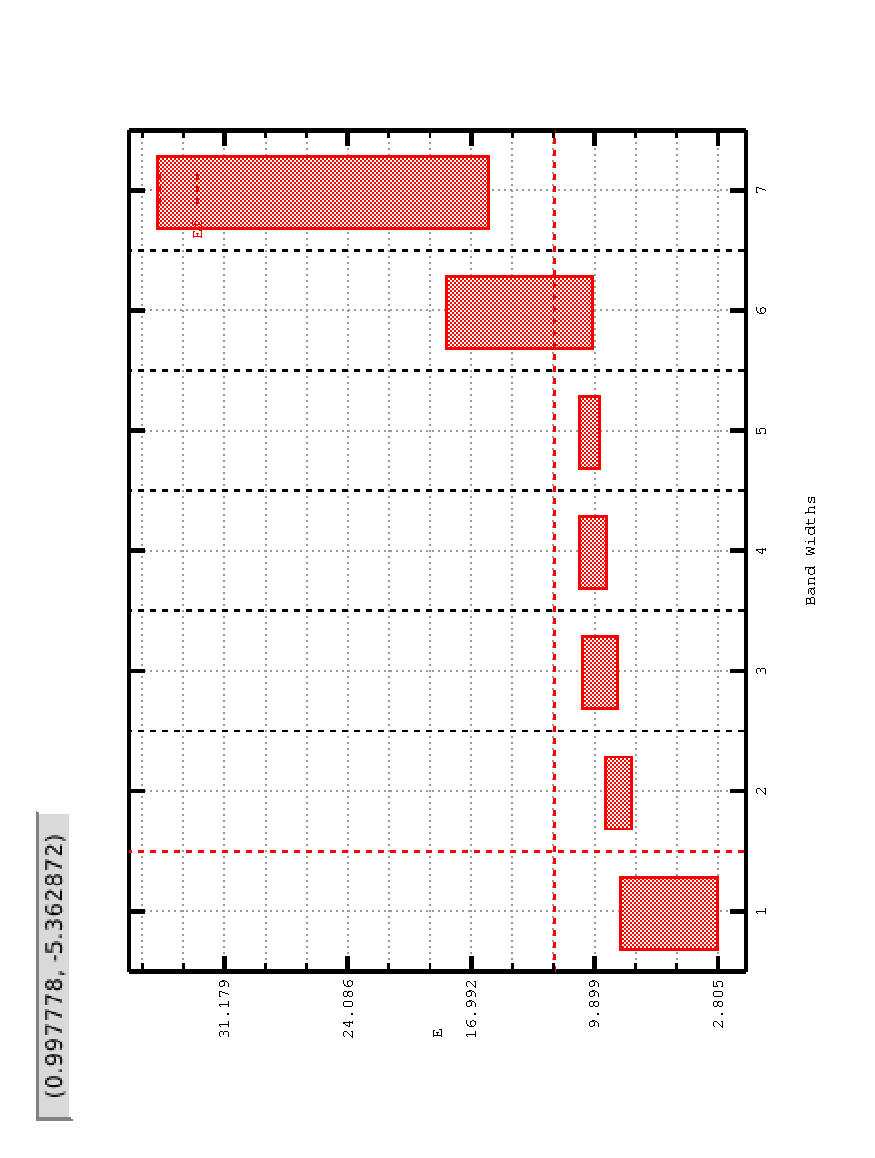
\includegraphics[width=0.35\columnwidth,trim={50pt 10pt 0pt 50pt},clip,rotate=270]{figure/example04/copper_bands_span.eps}}
	\centering
	\subfloat[Fermi surface]{\raisebox{-2.2in}{\rotatebox[origin=t]{0}{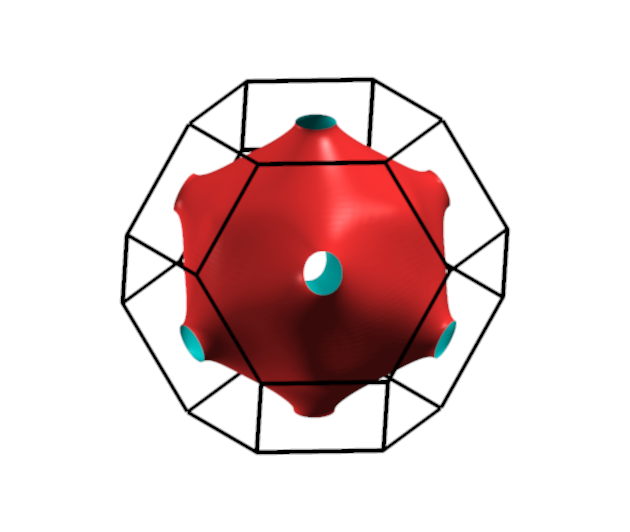
\includegraphics[width=0.35\columnwidth,trim={10pt 10pt 10pt 10pt},clip]{figure/example04/copper_fermi.png}}}}
	\caption{Fermi surfaces for band 6 in copper. The value of the Fermi energy is 12.2103\eV, and it was obtained from DFT calculation, with a $4\times4\times4$ \bfk-point mesh. To calculate the band energies and to plot Fermi surfaces, Wannier interpolation was employed on a dense mesh in the Brillouin zone consisting of $50^3$ points.}\label{fig4.1}
	\end{figure}
	\item {\it Plot the interpolated bandstructure.}

	Interpolated bandstructure, with path in k-space given in the tutorial,  is shown in \Fig{fig4.2}.
	\begin{figure}[t!]
	\centering
	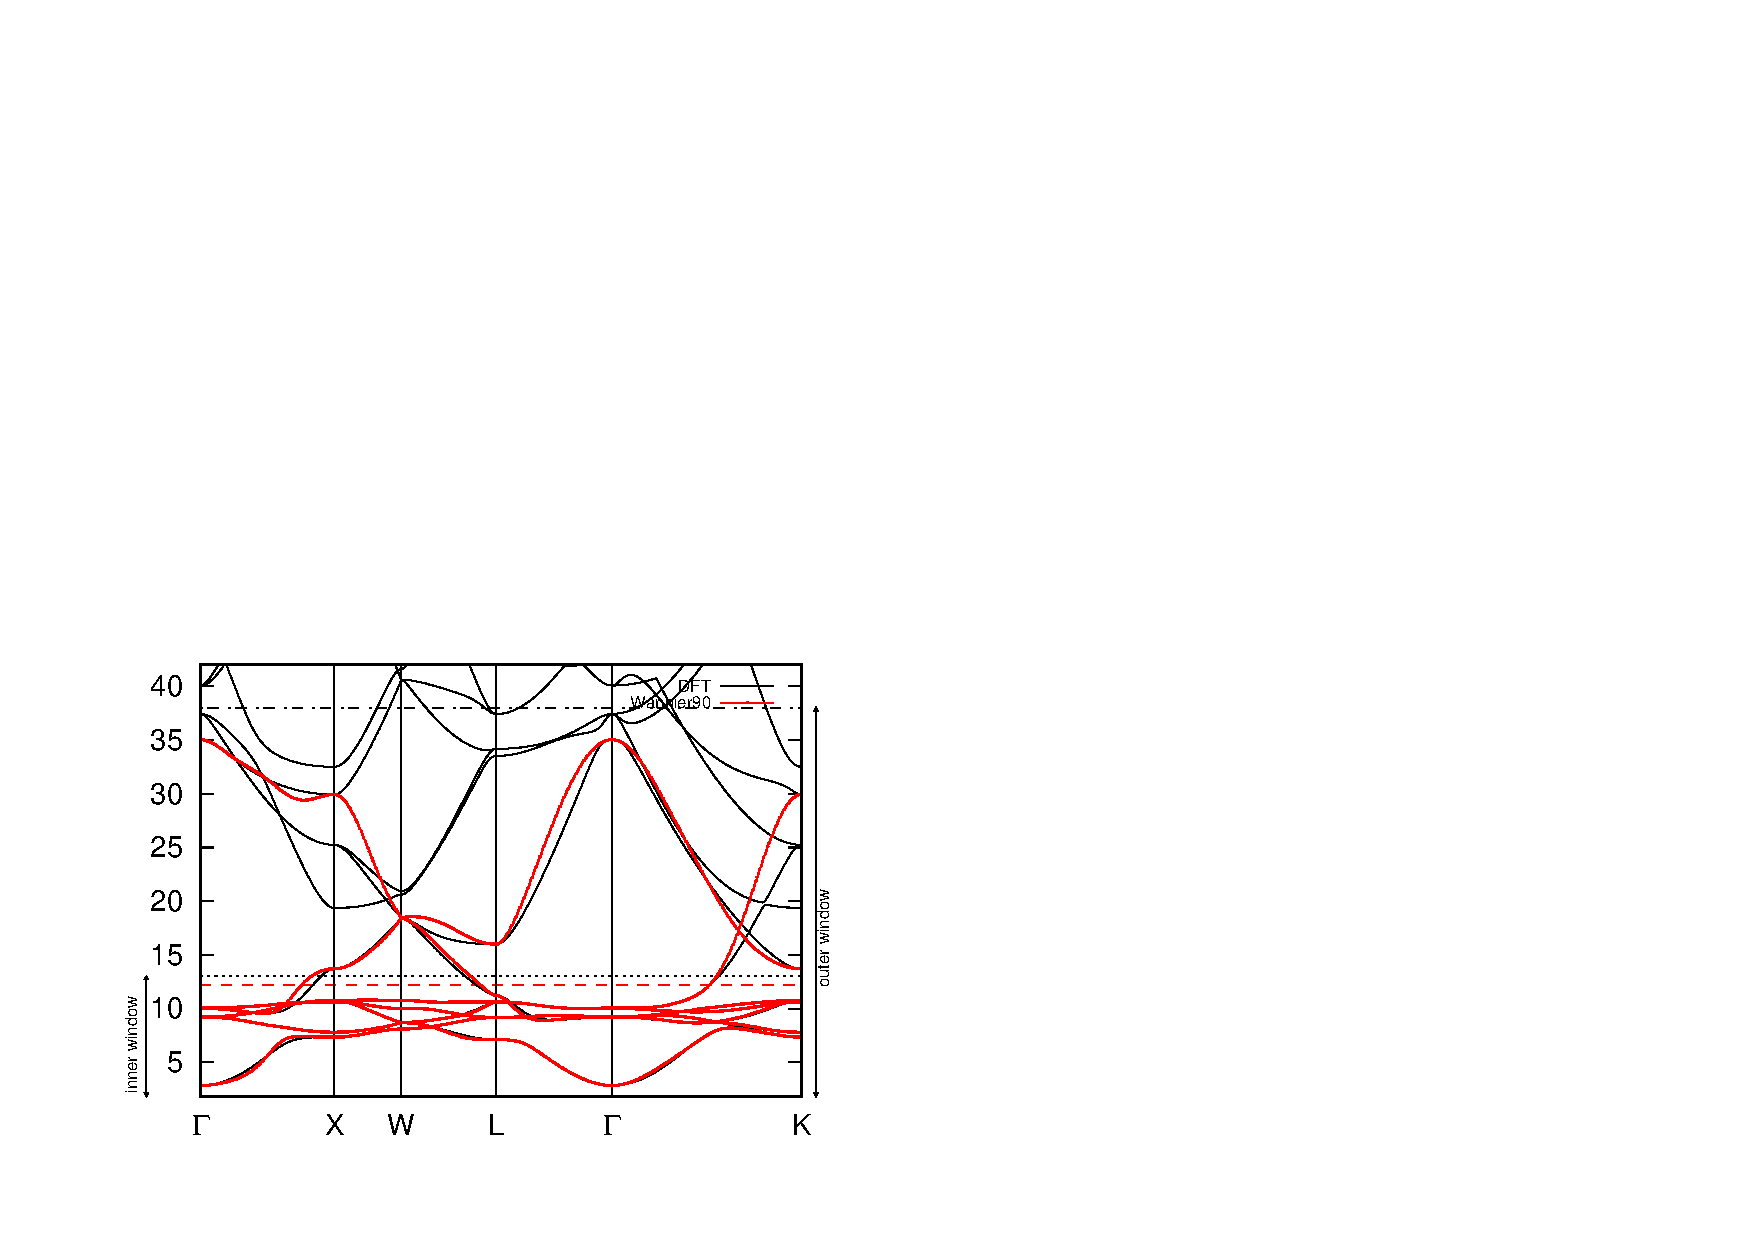
\includegraphics[width=0.8\columnwidth,trim={10pt 10pt 400pt 300pt},clip]{figure/example04/copper_bs_qe_w90}
	\caption{Interpolated bandstructure of Copper (solid red) showing the position of the Fermi level (dashed red) and both inner and outer windows (dotted and dashed-dotted respectively). The reference DFT bandstructure (solid black) was obtained with Quantum ESPRESSO, see procedure in Example \protect\ref{sec6:copper}.}\label{fig4.2}
	\end{figure}
	\item  {\it Plot the contribution of the interstitial WF to the bandstructure.}

	The contribution of the 2 $s$-like \MLWFs{} to the band structure is shown in \Fig{fig4.3}
	\begin{figure}[h!]
	\centering
	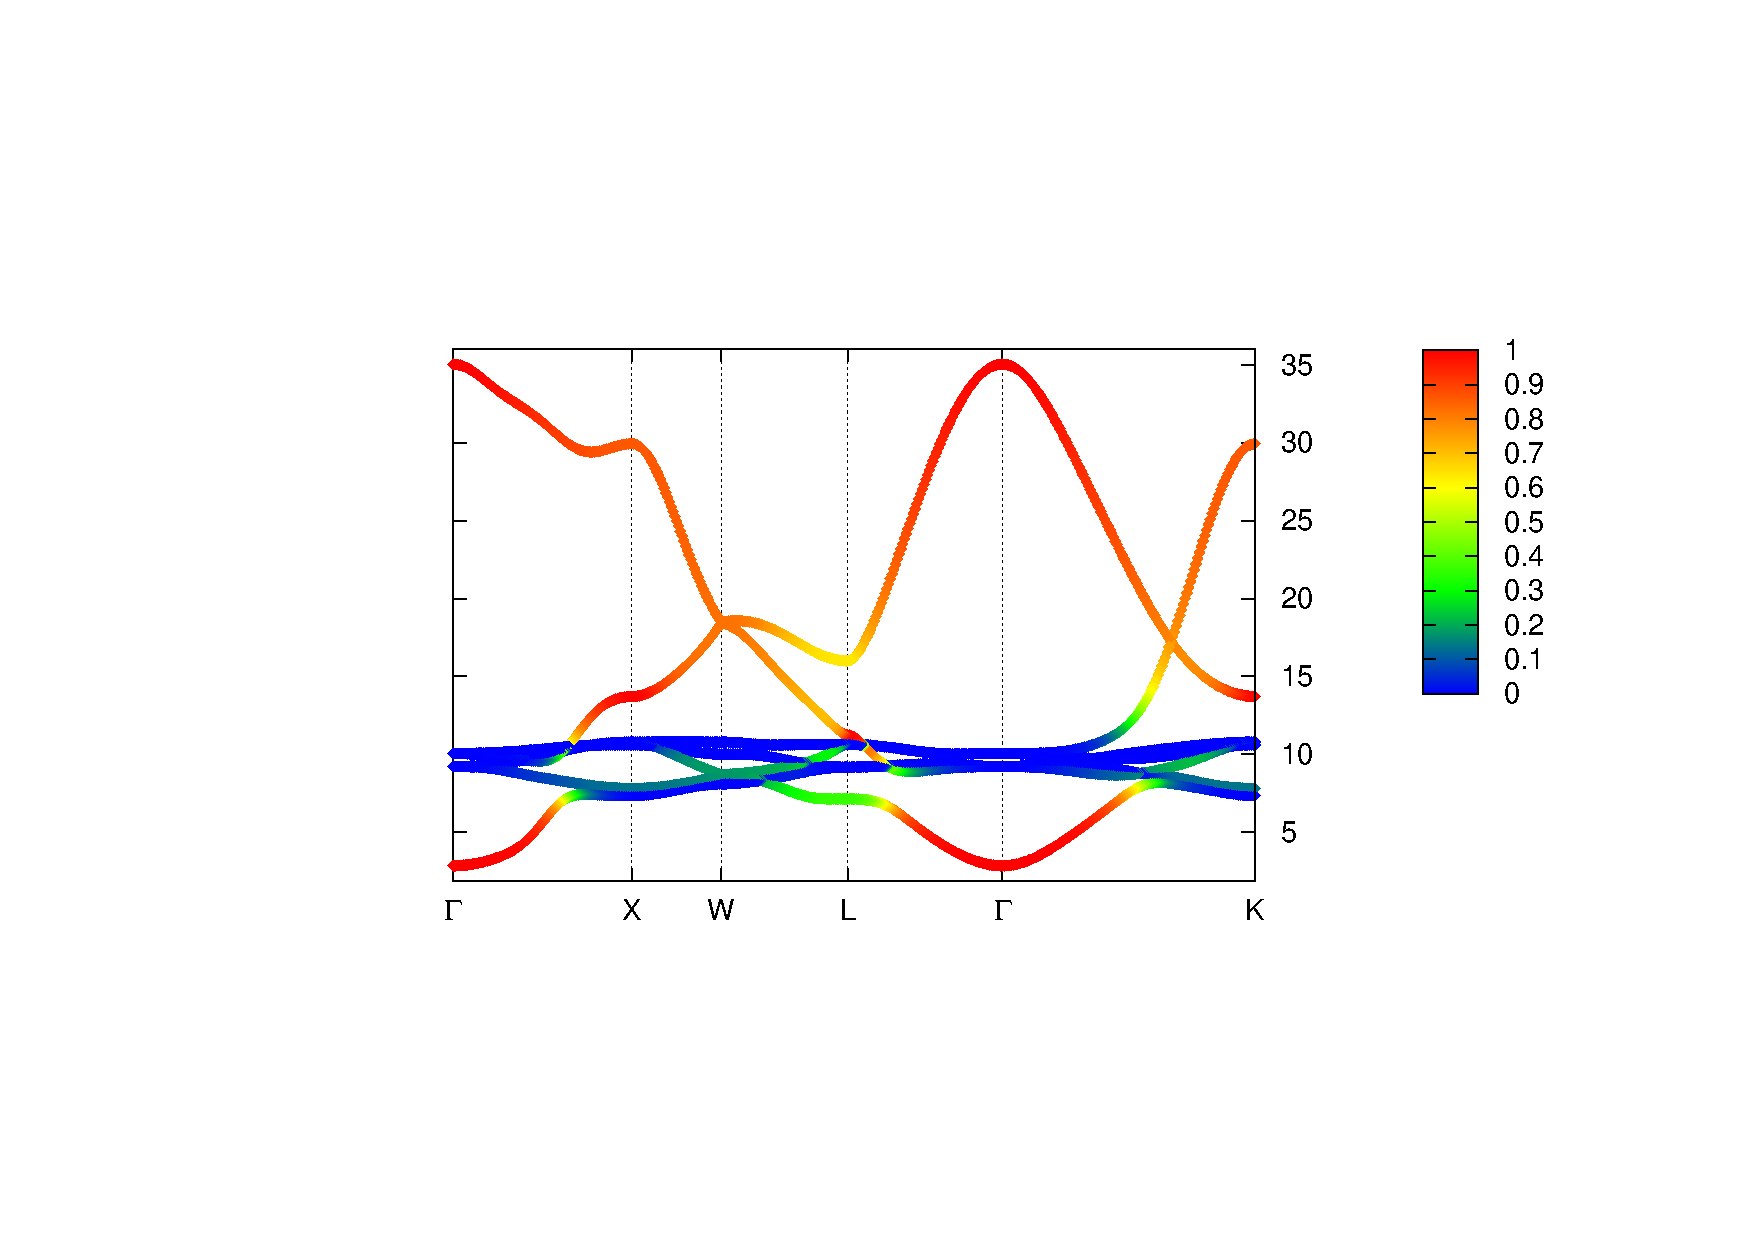
\includegraphics[width=0.9\columnwidth,trim={120pt 120pt 80pt 100pt},clip]{figure/example04/copper_bs_projection}
	\caption{Bandstructure of Copper showing the contribution from the 2 $s$-like \MLWFs{} in red.}\label{fig4.3}
	\end{figure}

	\item[Extra :] {\it Investigate the effect of the outer and inner energy window on the interpolated bands.}

	From now on, we will refer to the inner window energy level as $\varepsilon_{\mathrm{in}}$ and to the outer window energy level as $\varepsilon_{\mathrm{out}}$. The reference values are in this case $\varepsilon_{\mathrm{in}}^0 = 13$eV and $\varepsilon_{\mathrm{out}}^0 = 38$eV. Hereafter, we will use $\varepsilon_{\mathrm{min}}$ to refer to the minimum energy eigenvalue (for the chosen path). The value of $\varepsilon_{\mathrm{out}}^0$ must be chosen such that there are at least $N_{\mathrm{wannier}}$ (7 in this case) states inside the outer energy window for each \bfk-point. This means that for a given path in the BZ there exists a lower bound to $\varepsilon_{\mathrm{out}}^0$. The actual value depends on the path in the BZ and on the choice of the zero for the pseudopotential. The result for several values of $\varepsilon_{\mathrm{in}}$ and $\varepsilon_{\mathrm{out}}$ are shown in \Fig{fig4.4}.


	\begin{figure}
	\centering
	\subfloat[$\varepsilon_{\mathrm{in}} = 5$eV, $\varepsilon_{\mathrm{out}}=\varepsilon_{\mathrm{out}}^0$]{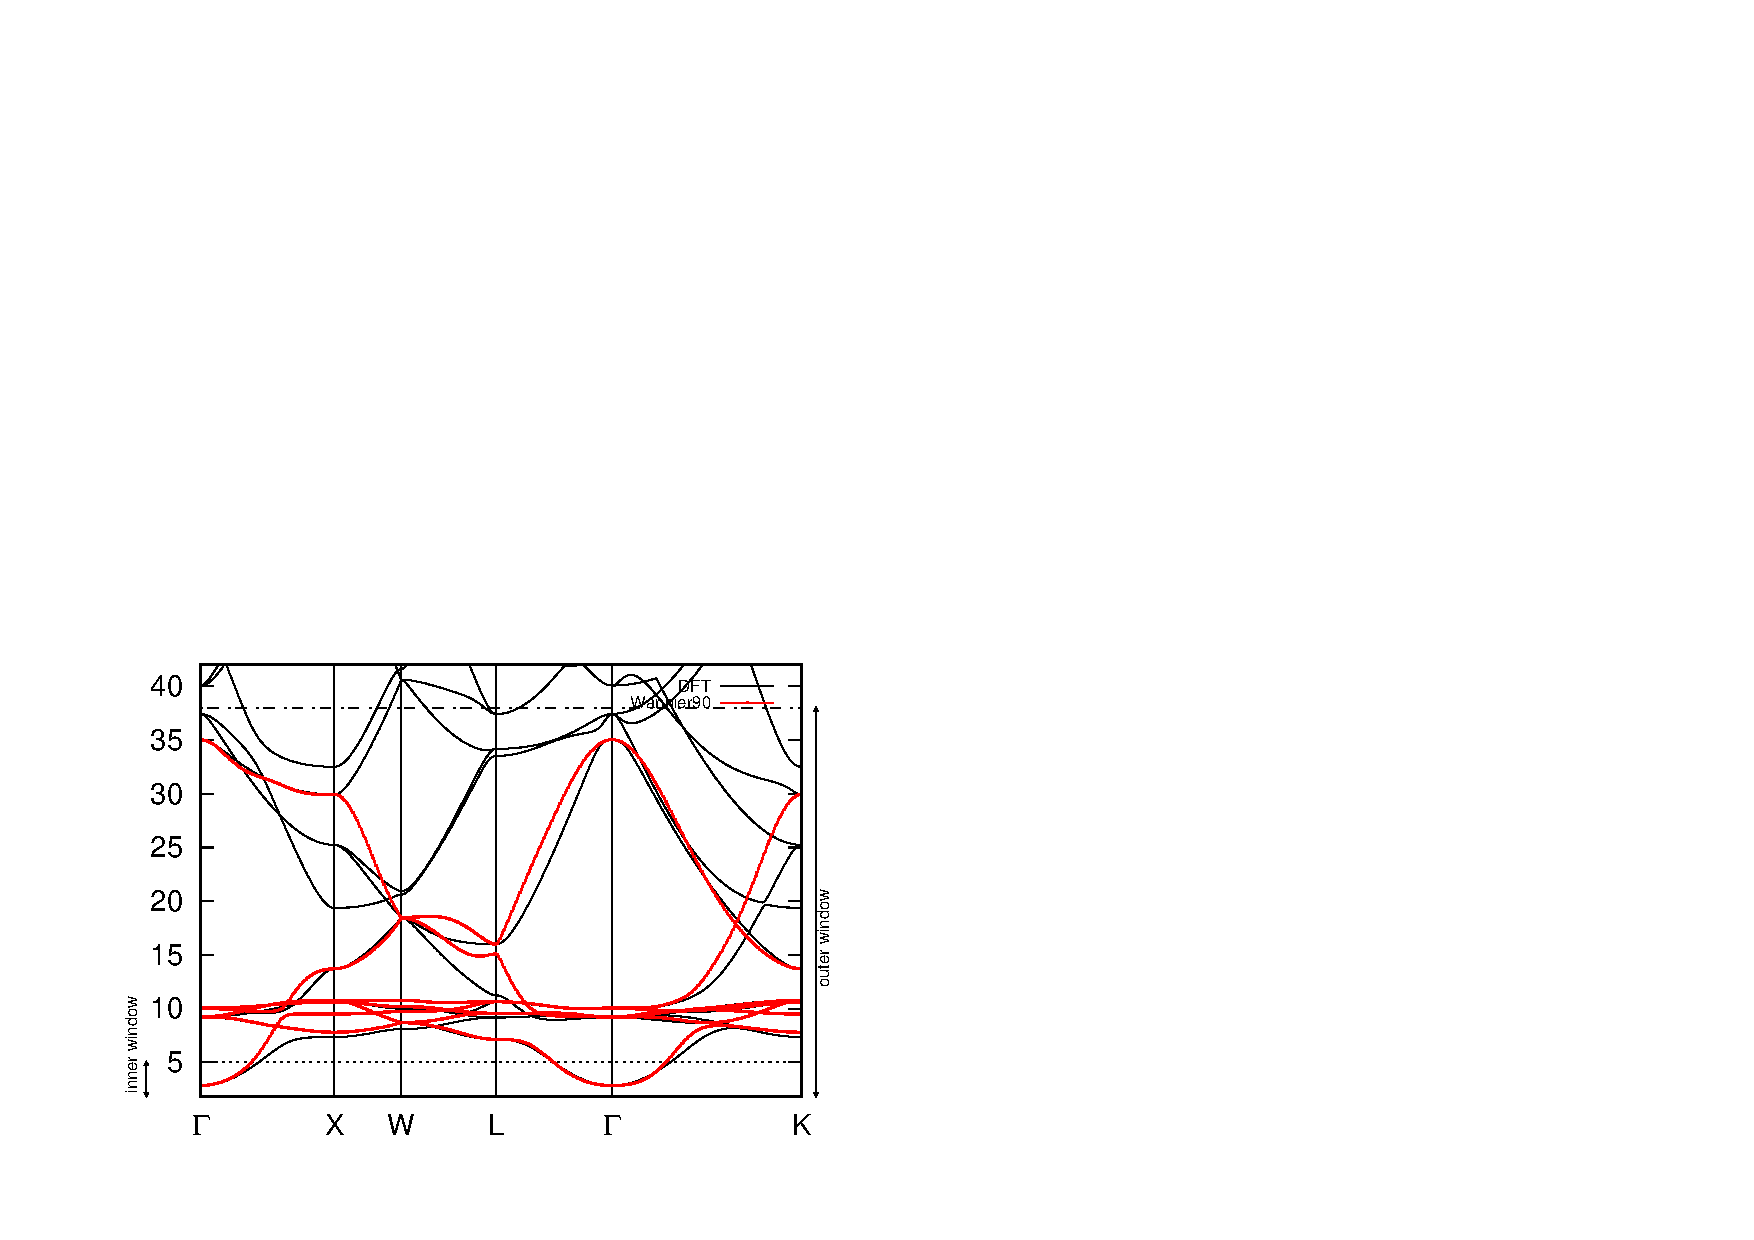
\includegraphics[width=0.49\columnwidth,trim={30pt 30pt 380pt 300pt},clip]{figure/example04/copper_bs_qe_w90_5_38}}
	\centering
	\subfloat[$\varepsilon_{\mathrm{in}} = 9.5$eV, $\varepsilon_{\mathrm{out}}=\varepsilon_{\mathrm{out}}^0$]{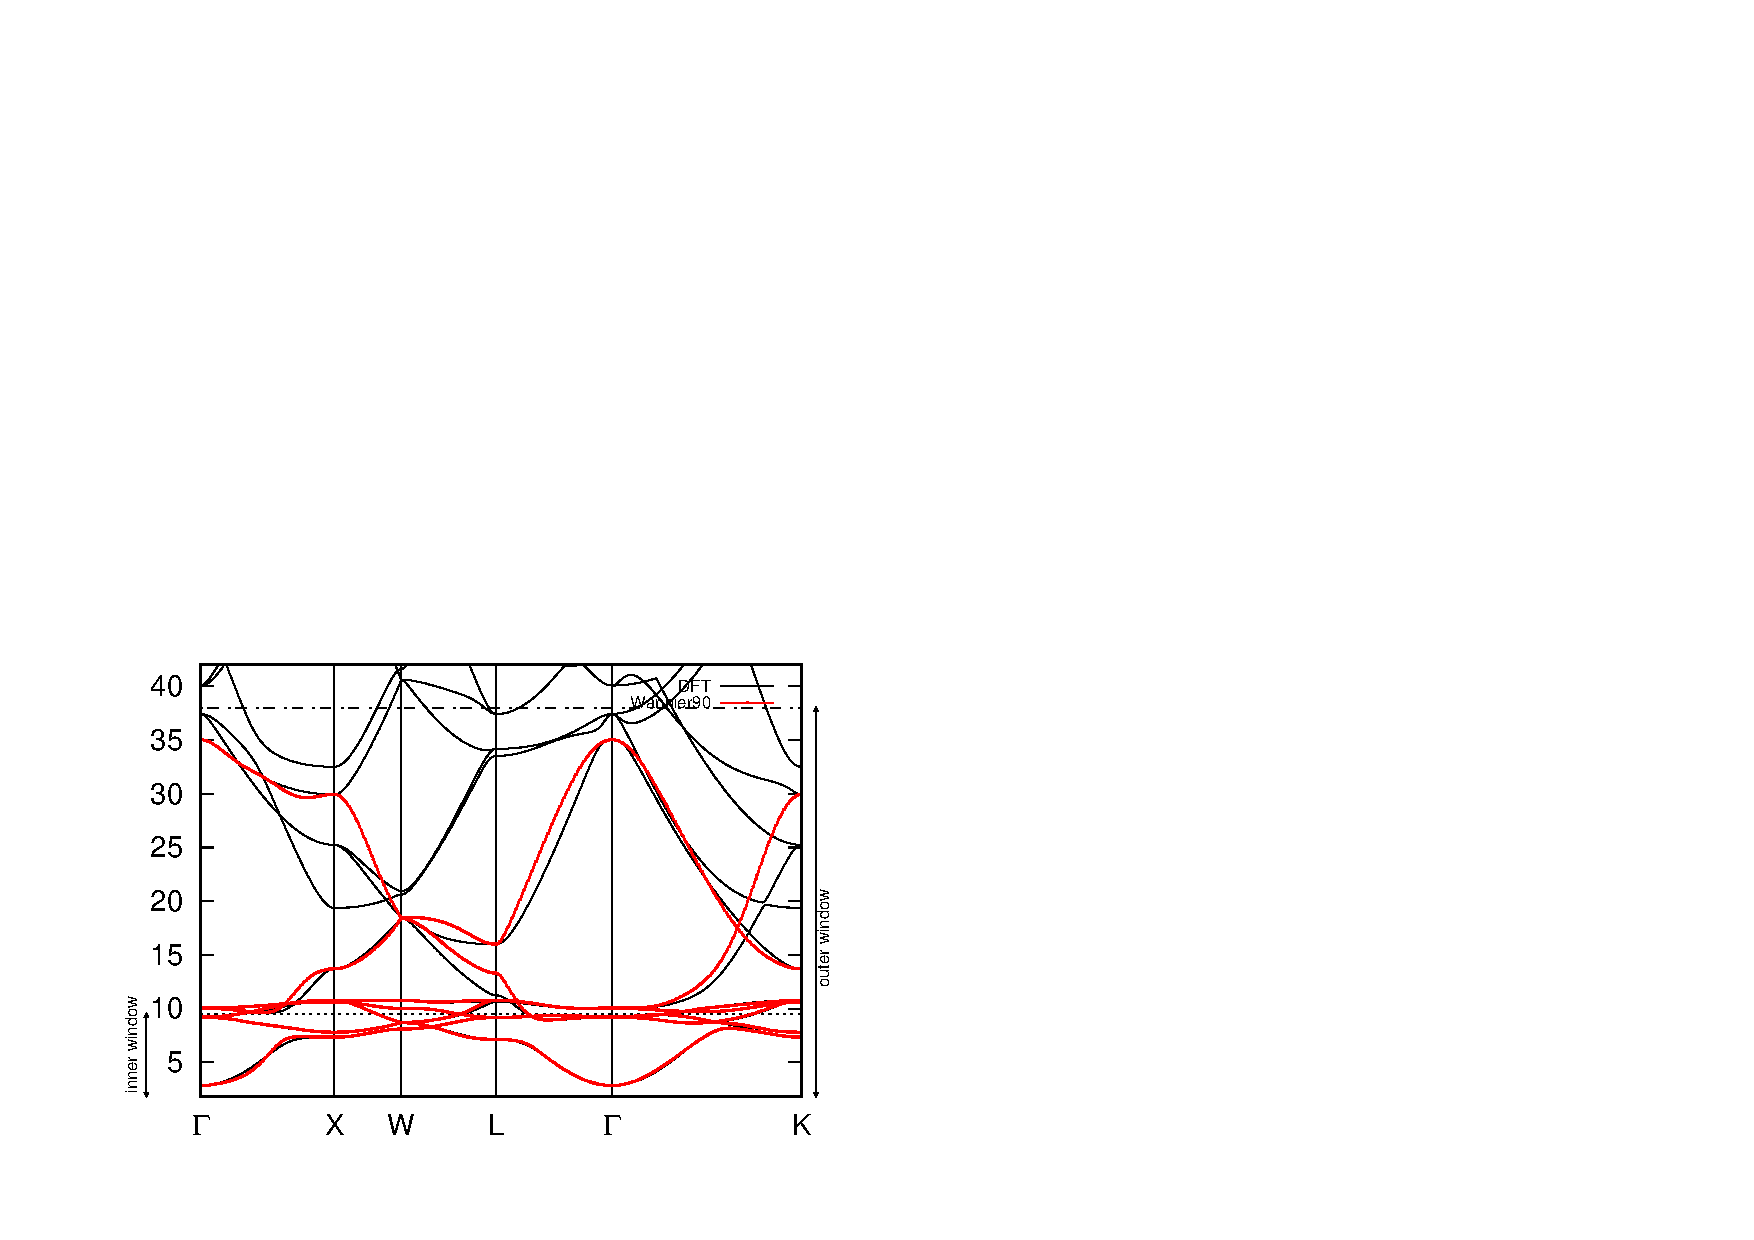
\includegraphics[width=0.49\columnwidth,trim={30pt 30pt 380pt 300pt},clip]{figure/example04/copper_bs_qe_w90_9-5_38}}\\
	\centering
	\subfloat[$\varepsilon_{\mathrm{in}} = \varepsilon_{\mathrm{in}}^0$, $\varepsilon_{\mathrm{out}}=\varepsilon_{\mathrm{out}}^0$]{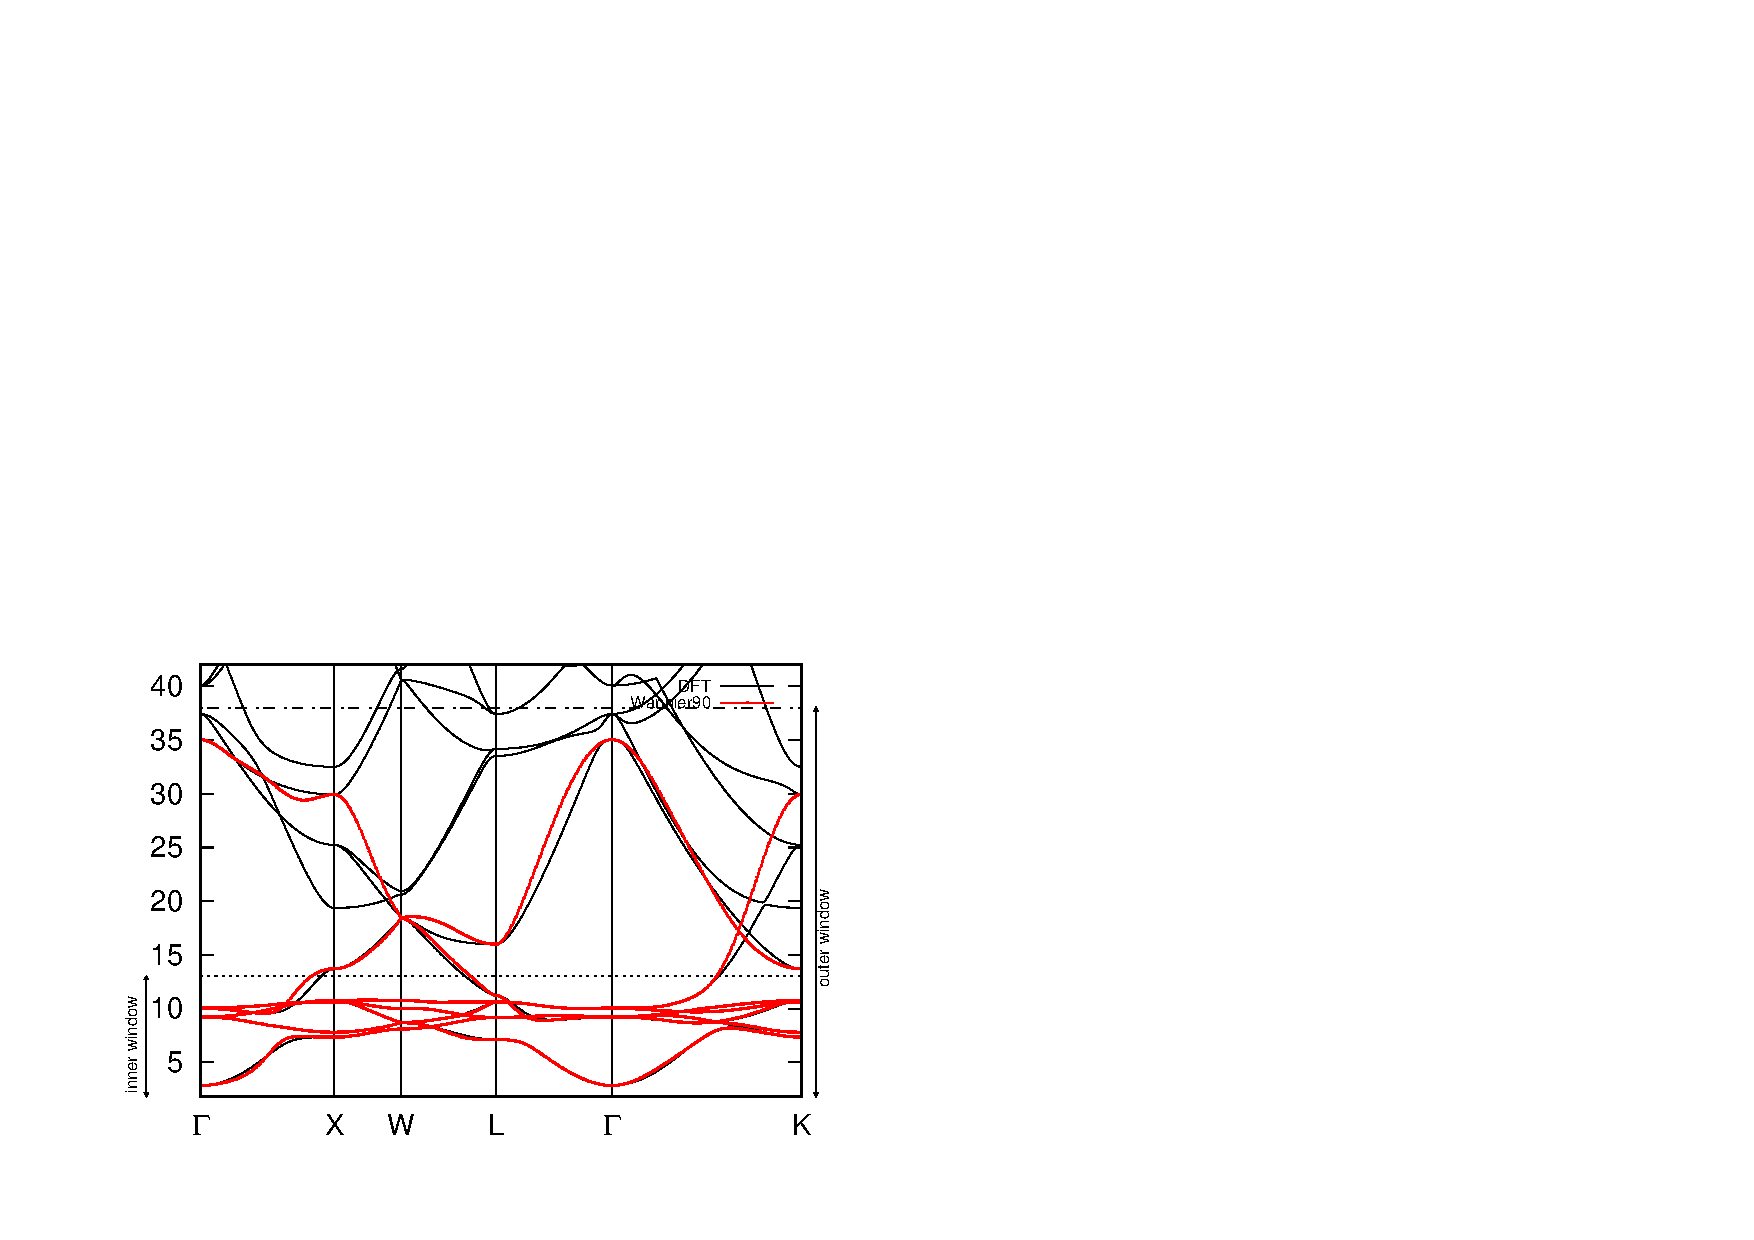
\includegraphics[width=0.49\columnwidth,trim={30pt 30pt 380pt 300pt},clip]{figure/example04/copper_bs_qe_w90_13_38}}
	\centering
	\subfloat[$\varepsilon_{\mathrm{in}} = 15$eV, $\varepsilon_{\mathrm{out}}=\varepsilon_{\mathrm{out}}^0$]{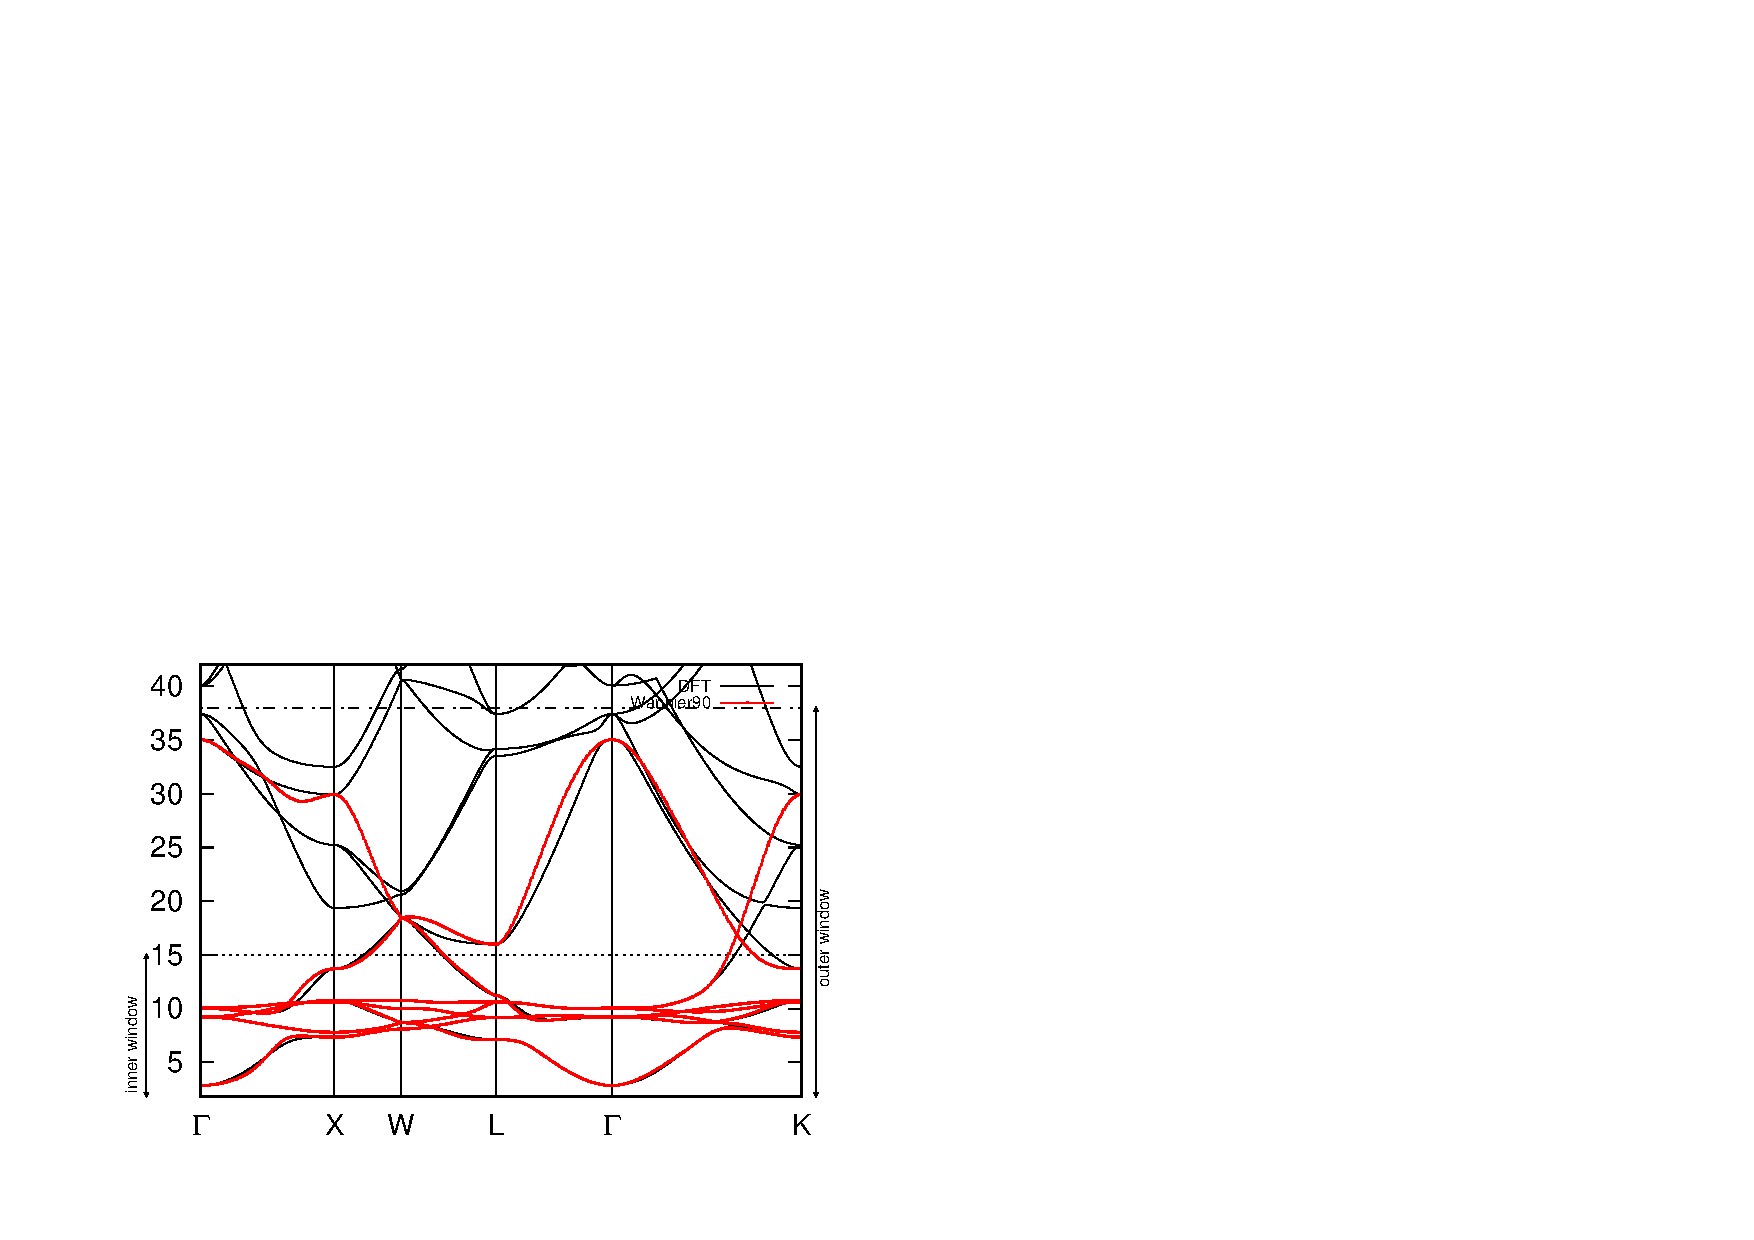
\includegraphics[width=0.49\columnwidth,trim={30pt 30pt 380pt 300pt},clip]{figure/example04/copper_bs_qe_w90_15_38}}\\
	\centering
	\subfloat[$\varepsilon_{\mathrm{in}}=\varepsilon_{\mathrm{min}}$, $\varepsilon_{\mathrm{out}}=\varepsilon_{\mathrm{out}}^0$]{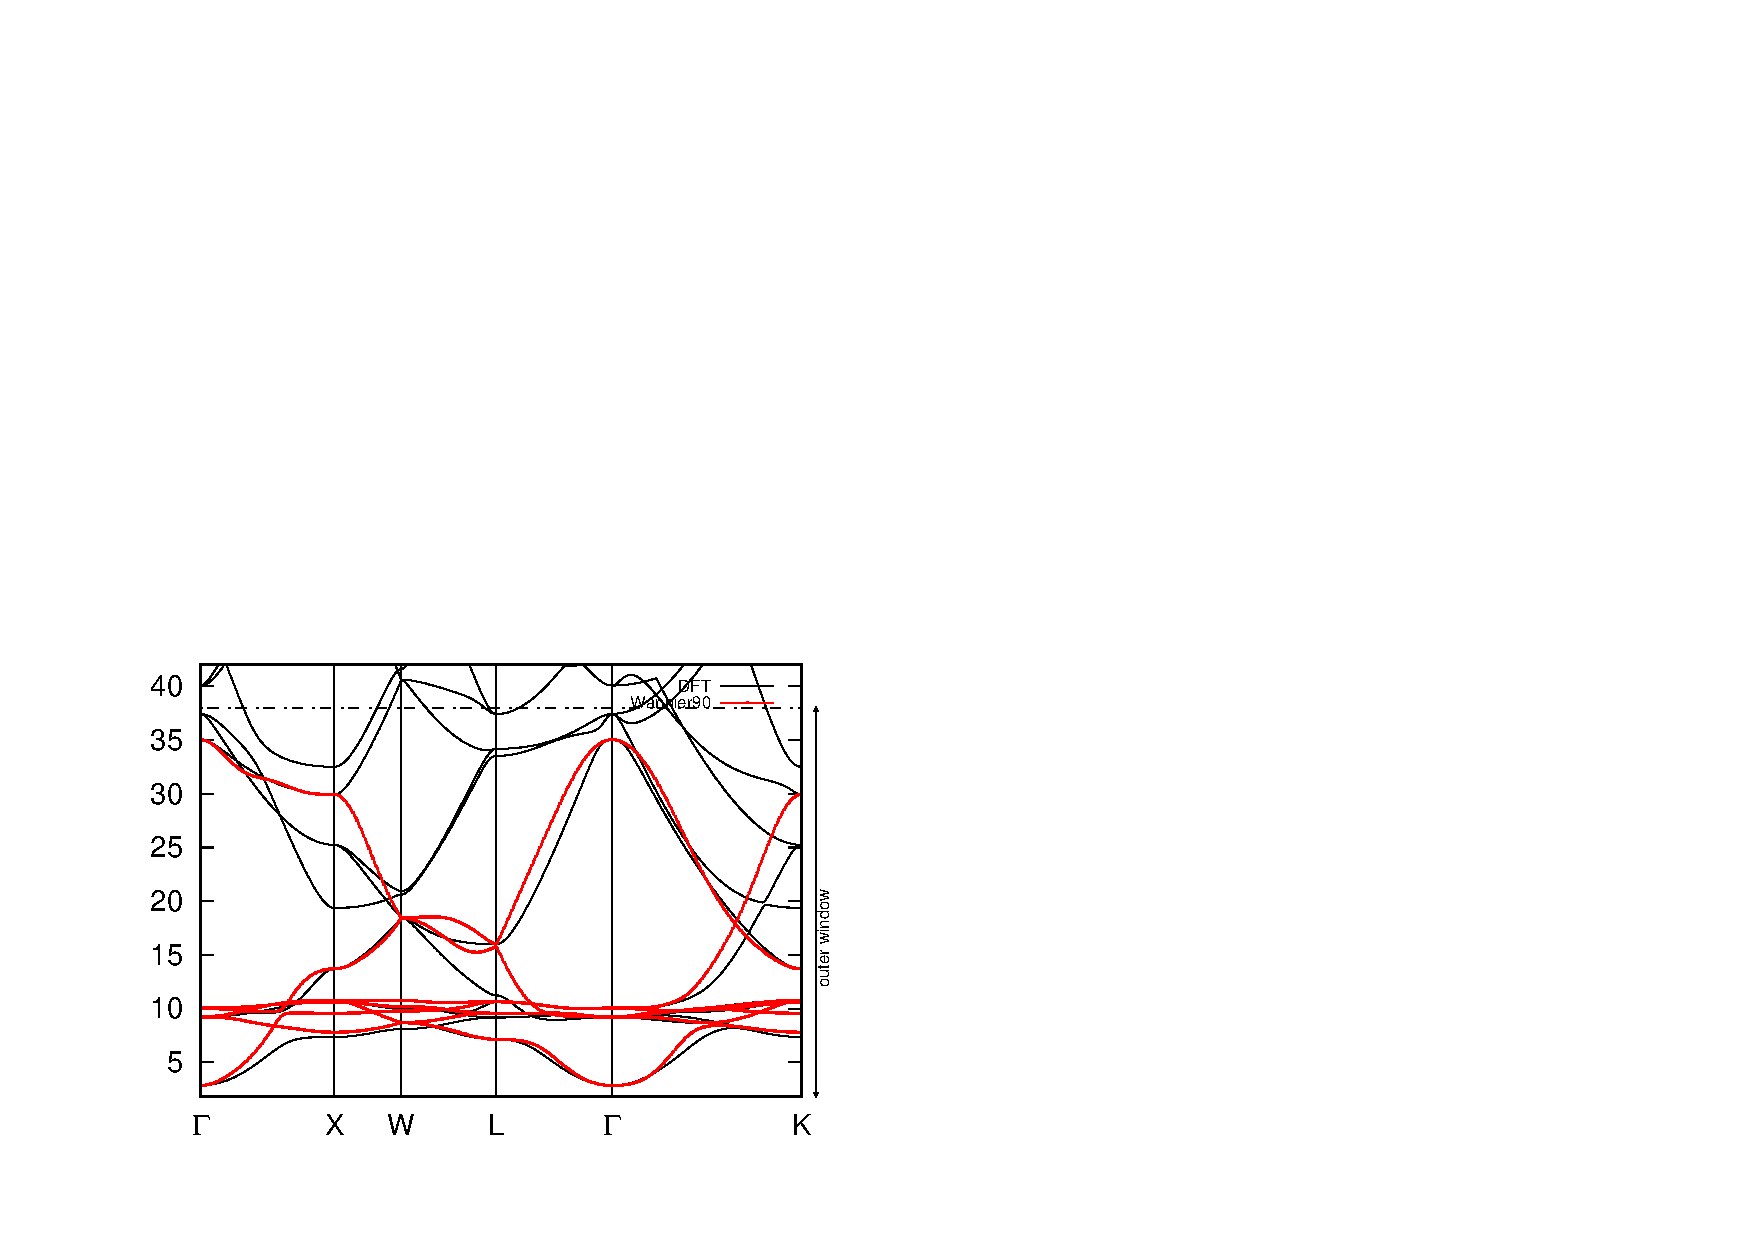
\includegraphics[width=0.49\columnwidth,trim={30pt 30pt 380pt 300pt},clip]{figure/example04/copper_bs_qe_w90_no_38}}
	\centering
	\subfloat[$\varepsilon_{\mathrm{in}}=\varepsilon_{\mathrm{min}}$, $\varepsilon_{\mathrm{out}}= 45$eV]{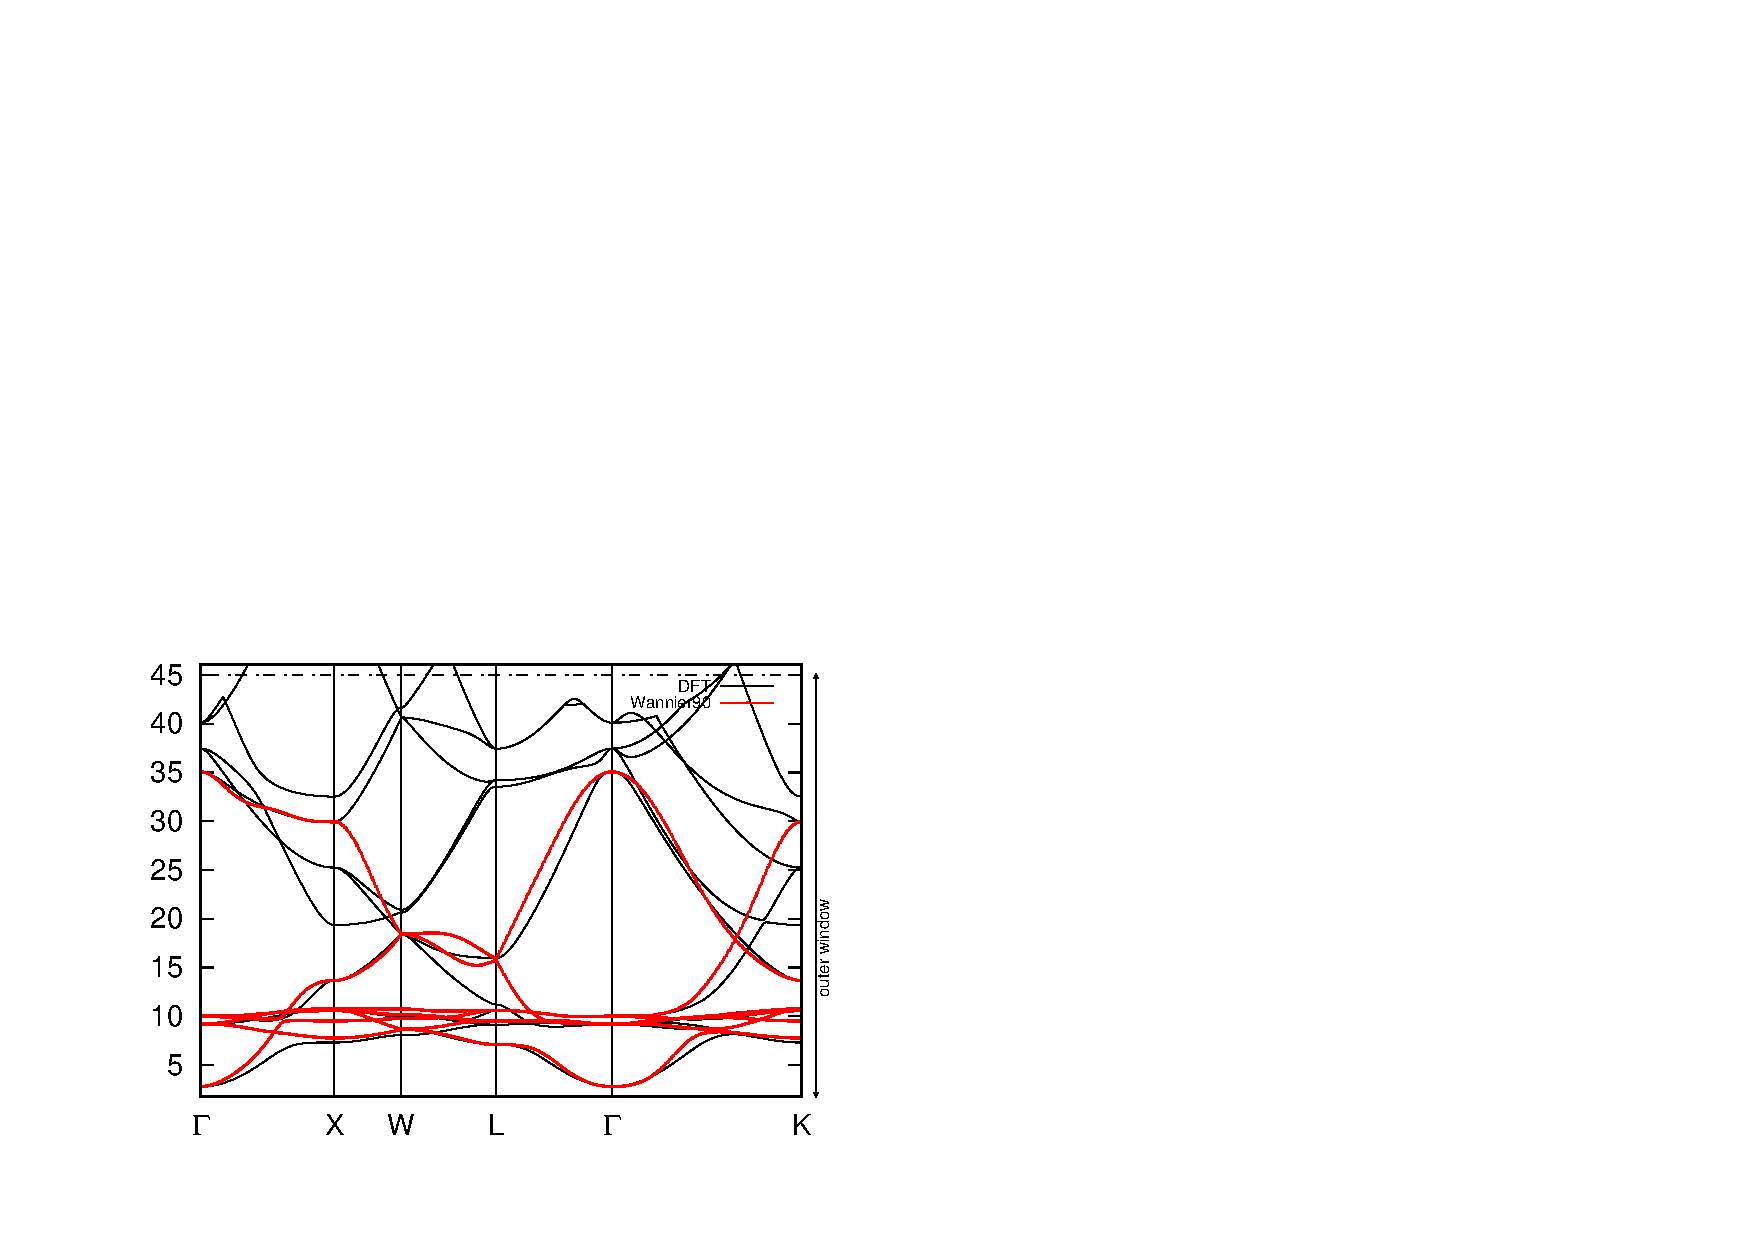
\includegraphics[width=0.49\columnwidth,trim={30pt 30pt 380pt 300pt},clip]{figure/example04/copper_bs_qe_w90_no_45}}
	\caption{Interpolated  bandstructure of Copper (solid red) with DFT reference (solid black) and different values of the inner window. Panel a) $\dots$  }\label{fig4.4}
	\end{figure}
\end{enumerate}
